\section{Ejercicio 3}

\subsection{Problema: Girls Scouts}
El capitan de Las Girasoles quiere evitar los problemas en el fogoon del ano anterior cuando las exploradoras rompieron en llanto por no poder sentarse en la ronda junto a sus mejores amigas. En secreto les asigno una letra a cada nina y relevo quien se llevaba con quien. \\
Su idea es organizar la ronda de manera que exista la menor distancia posible entre cada amistad. \\

Con esto se sabe que trabajara con un conjunto de personas y un conjunto de amistades entre ellos, para esto decidimos modelar al conjunto de personas como un arreglo para determinar las posiciones que tendran cada una. Por otro lado las combinaciones de posibles lugares a saltarce simplemente seran permutaciones del arreglo. \\

La entrada consta de un conjunto de personas y sus respectivas amistades(las cuales tambien perteneceran al conjunto). Se quiere que, al sentarlas a todas en una ronda, se minimize la suma de distancias entre todos los pares de amistades dentro de la misma.
%en tiempo estrictamente menor a $\bigO (e^e . a^2)$ \par

\subsubsection{Ejemplos}

\begin{table}[htb]
\centering
\begin{tabular}{|l|l|}
\hline
Linea Entrada                    & Linea Salida \\ \hline
a bcde;b acde;c abde;d abc;e abc & 2 abdce      \\ \hline
a bcd;b ae;c ad;d ac;e b         & 2 abecd      \\ \hline
a fb;b gc;d gc;f agh;e hd        & 3 abgcdehf   \\ \hline
x yz                             & 1 xyz        \\ \hline
\end{tabular}
\caption{Ejemplos Girls Scouts}
\label{my-label}
\end{table}



\subsection{Desarrollo}
Dado que no es necesario generar las permutaciones que incluyan elementos repetidos, dado $e$ un conjunto de personas, si genero permutaciones con elementos repetidos tendria $e^e$ posibles combinaciones(ya que tendriamos $e$ posibilidades para la primer posicion, $e$ para la segunda y asi hasta la $e-esima$ posicion). A la hora de generar permutaciones sin repeticion de elementos tendremos $e$ posibilidades en la primera posicion, $e-1$ en la segunda y asi susecivamente hasta la llegar a la $e-esima$ posicion donde solo nos quedara una posibildad. De esta manera redujimos el espacio de permutaciones posibles a:
\newline

\begin{center}
    \underline{$e$}
    \underline{$e-1$}
    \underline{$e-2$}
    \underline{$e-3$}
    \underline{$. . .$}
    \underline{$1$} \newline
    Posibles combinaciones \newline \newline
    $= e * (e - 1) * (e - 2) * ... * 1$ \newline \newline
    $= \prod_{i = 1}^e i$ \newline \newline
    $= e!$ \newline
\end{center}
 
De esta manera se genera primero la permutacion inicial(con los elementos ordenados lexicograficamente, ej: a,b,c,d,e) y luego se crearan nuevas permutaciones quedandose siempre con la que cumpla las condiciones (es importante notar que el calculo de la suma de distancias se hara solo al momento que la permutacion sea generada en su totalidad, mas adelante se entrara en detallle sobre este aspecto). Como no es necesario calcular todas las permutaciones al mismo tiempo para luego compararlas, se iran creando de a una y solo se mantendra la mejor hasta el momento, evitando asi tener mayor costo espacial.

\subsection{Justificaci\'on y Complejidad}
Como explicamos recien, vamos a tener $e!$ permutaciones para revisar. Para cada una de estas permutaciones, lo que vamos a hacer es calcular la suma de la longitud de las exploradoras que estan relacionadas por una amistad. A este proceso lo llamaremos calcular el $costo$ de la ronda.\par

\begin{description}
  \item[Algoritmo 3.1 Caso base (creacion de Ronda)] \hfill \\
  \begin{verbatim}
    rondaAGuardar <- copiarRonda(rondaActual); O(e)
    calcularDistancias(rondaAGuardar); O(e^3)
   \end{verbatim}
\end{description}

\begin{center}
\newline
$ \bigO(e + e³) $ \newline \newline
$ \bigO(e³) $ \newline \newline
\end{center}
Con esto tenemos costo cubico para crear una ronda, veamos las complejidades de calcularDistancias: \newline

\begin{description}
  \item[Algoritmo 3.2 calcularDistancias] \hfill \\
  \begin{verbatim}
    sumaDistancias  <- 0
    AmigaMasLejana  <- 0 
    FOR i <- 0 to ronda.length  O(e)
        mejoresAmigas <- ronda[i] O(1)
        posNina <- obtenerPos(mejoresAmigas[0]) O(e)
        j <- 2
        WHILE j < mejoresAmigas.length() O(a)
            posicionAmiga   <- obtenerPos(mejoresAmigas[j]) O(e)
            distancia       <- absoluto(posNina - posicionAmiga) O(1)
            distanciaMinima <- minimo(distancia, ronda.length - distancia) O(1)
            sumaDistancias  <- sumaDistancias + distanciaMinima; O(1)
            if (amigaMasLejana > distanciaMinima) amigaMasLejana <- distanciaMinima O (1)
            j++
        ENDWHILE
    ENDFOR
    return <- res
    \end{verbatim}
\end{description}

\begin{center}
    $\sum_{i = 1}^e ( e + \sum_{i = 1}^{a_i} e )$ \newline \newline
    con $e$, cantidad de personas en la ronda y $a_i$, cantidad de amigas de la $i-esima$ persona \newline \newline
Como la cantidad de amigas puede ser a lo sumo $e$ se puede acotar por\newline \newline
    $= \sum_{i = 1}^e ( e + \sum_{i = 1}^{e} e )$ \newline  \newline
    $= \sum_{i = 1}^e ( e + e^2 )$ \newline \newline
    $= e * ( e + e^2 )$ \newline \newline
    $ \bigO(e² + e³ )$ \newline \newline
    $ \bigO( e³ )$ \newline
\end{center}

Calculada la complejidad del caso base pasemos a ver el caso general:

\begin{description}
  \item[Algoritmo 3.3 parametros: ronda, permutacion] \hfill \\
  \begin{verbatim}
mejorRondaActual <- mejorPermutacion(ronda, permutacion + 1);
FOR i <- permutacion + 1; i < ronda.length; i++  O(e - permutacion)
    swap(ronda, permutacion, i); O(1)
    mejorRondaPermutada <- mejorPermutacion(ronda, permutacion + 1);
    swap(ronda, permutacion, i); O(1)
    
    if (mejorRondaPermutada.sumaDistancias < mejorRondaActual.sumaDistancias)  O(1)
    	mejorRondaActual = mejorRondaPermutada; O(1)
    else
    
        if (mejorRondaPermutada.sumaDistancias ==  mejorRondaActual.sumaDistancias  
            AND (comparar(mejorRondaPermutada, mejorRondaActual)) )O(e)
            	mejorRondaActual = mejorRondaPermutada; O(1)
        ENDIF
    ENDIF
ENDFOR
return <- mejorRondaActual
    \end{verbatim}
\end{description}

\begin{center}
Veamoslo paso a paso, en el primer caso de entrada el bucle tendra $e-1$ repeticiones de costo $e-1$ cada una pero como forzamos una llamada antes de entrar al mismo, quedan $e$ lladas de costo $e-1$, la segunda vez sera analoga con $e - 1$ repeticiones, la tercera $e - 2$ y asi sucesivamente. Si defino la funcion de recurrencia queda: \newline

 $T(e)= \left\{ \begin{array}{lcc}
             e * T(e-1)&   si  & e\ $>$\ 1 \\
             \\ 1 &  si  & e\ $=$\ 1
             \end{array}
   \right.$
\end{center} 
Por el momento no tengamos en cuenta el costo $e$ de cada bucle para comparar las rondas, veamos solo que cantidad de llamadas tendremos.  \newline

\begin{center}
$ T(e) = e * T(e - 1)$ \newline \newline
$= \prod_{i = 1}^e i $ \newline \newline
$= e! $ \newline \newline
\end{center}

Por lo que la copmlejidad de la recursion sera $e!$ agregandole $e$ por cada llamada nos queda $\bigO(e! * e)$, a continuacion se agregaran los casos bases suponiendo que ocurren siempore (cosa que en realidad solo pasa en las hojas del arbol del recursion). \newline \newline

\begin{center}
    $= \bigO(e! * e * e^3)$ \newline \newline
    $= \bigO(e! * e^4)$ \newline \newline
\end{center}

Ahora veamos que cumple con la complejidad pedida(por simplicidad solo escribiremos el contenido de la complejidad) \newline \newline

\begin{center}
    $e^e * a^2 > e! * e^4$ \newline \newline
    
    tomando el primer termino \newline \newline
    
    $e^e * a^2 > e^e$ \newline \newline
    
    veamos si $e^e > e! * e^4$ \newline \newline
    
    $e^{e-4} * e^4 > e! * e^4$ \newline \newline
    
    $e^{e-4} > e!$ \newline \newline
    
    expandiendo ambos terminos \newline \newline
    
    $e * e * e ... * e > e * (e-1) * (e-2) * ... * 5 * 4 * 3 * 2 * 1$  \newline \newline
    
    Como $4*3*2*1$ es constante puede ser eliminado de la ecuacion \newline \newline
    
    $e * e * e ... * e > e * (e-1) * (e-2) * ... * 5$ \newline \newline
    
    Ahora cada termino tiene exactamente $e-4$ elementos, basta ver que solo el primero es igual ($e$) y el resto son todos menores del lado derecho. De esta manera: \newline \newline
    
    $e * e ... * e > (e-1) * (e-2) * ... * 5$ \newline \newline
    
    Luego  \newline \newline
    
    $\bigO(e^e * a^2) > \bigO(e^e) > \bigO(e! * e^4)$ \newline \newline
    
    $\bigO(e^e * a^2) > \bigO(e! * e^4)$ \newline \newline
    
    Que es lo que queriamos demostrar. \newline
    
\end{center}

\subsection{Correctitud}
Como dijimos Previamente existen $e!$ combinaciones posibles de elementos sin repetir y el algoritmo las recorre todas. Como se puede ver en el algoritmo 3.3 por cada entrada recorre desde la posicion $permutacion$ hasta el final de la ronda swapeando el elemento actual del bucle contra la posicion de la permutacion, llama a la recursion y cuando vuelve lo swapea al lugar donde estaba previamente para probar swapear en el siguiente en la proxima iteracion, de esta manera en el primer caso de la recursion intercambiara el primer elemento del arreglo con todo el resto, dejara ese estatico y en el proximo paso recursivo intercambiara a partir del segundo elemento contra todos los siguientes y asi hasta llegar al ultimo elemento que quedara estatico y esa sera una posible solucion. Con esto quedan generadas todas las posibles permutaciones ya que el primer elemento se prueba en $e$ posiciones, el segundo en $e-1$ posiciones (ya que fue probado en el primer lugar cuando fue swapeado con el primero durante su iteracion) y asi sucesibamente.  \newline
Ahora veamos que calcula correctamente la suma de distancias y la distancia maxima entre amigas. El algoritmo 3.2 recorre todas las personas y todas las amigas de esas personas por lo que acarrea al maximo hasta terminar toda la busqueda con lo que efectivamente lo encuentra y la suma de distancias suma siempre la distancia minima entre dos amistades(3.2). Como recorre todas las combinaciones de amistades en la ronda podemos decir que su implementacion es correcta.
\newline
Veamos si el algoritmo acarrea la mejor solucion, en 3.3 podemos ver que luego de llamar a la recursion dentro del arreglo, se chequea contra la mejor hasta el momento (en el primer caso se compara contra la ronda sin modificaciones de esta recursion, la cual por la llamada recursiva previa al bucle fuerza a generar la primer rama de la recursion) y, de ser menor estricto en suma de distancias simplemente se queda con ese.
De ser iguales en suma de distancias compara cual es menor lexicograficamente y de ser asi, cambia la mejor hasta el momento por la nueva permutacion, la cual se ira acarreando hasta que ocurra una mejor.
De esta manera podemos concluir que el algoritmo resuelve el problema propuesto como queriamos ver.

\subsection{Tests}

En este ejericio, el mejor y peor caso es mas evidente y mas sencillo que el anterior, como en nuestro algoritmo, siempre vamos a generar todas las permutaciones posibles, podando solo los casos con elementos repetidos, la unica funcion variante va a hacer la del costo, y como esta es $\bigO(e * a)$ , podemos notar que esta muy ligado a la cantidad de amistades presentes.
    \subsubsection{Mejor Caso}
      El mejor caso seria que no haya ninguna amistad, pero para tener un analisis un poco mas realista, asumimos que nuestro mejor caso es que solo exista una sola amistad, para que el algoritmo tenga un poco mas de sentido.
    \lstinputlisting[language=Java]{modulos/Tests_Code/testej3mejor.txt}
    \subsubsection{Peor Caso}
        El peor caso siguiendo el hilo en el que veniamos, seria que todas las exploradoras sean amigas entre si, que aunque todas las soluciones tienen el mismo costo, por la forma en que el algoritmo funciona, este es nuestro peor escenario. 
 \lstinputlisting[language=Java]{modulos/Tests_Code/testej3peor.txt}
 
\pagebreak

\subsubsection{Performance}

Para la siguiente tabla de tiempos, siguiendo la definici\'on que dimos de nuestros mejores y peores casos, pasamos a ver como se diferencian gr\'aficamente.

\begin{table}[htb]
\centering
\begin{tabular}{|l|l|l|}
\hline
 Peor Caso	& Mejor Caso & N \\ \hline
198 & 182 & 1 \\ \hline
108 & 95 & 2 \\ \hline
253 & 216 & 3 \\ \hline
765 & 406 & 4 \\ \hline
1431 & 1245 & 5 \\ \hline
2845 & 2678 & 6 \\ \hline
14181 & 10159 & 7 \\ \hline
89646 & 48423 & 8 \\ \hline
1255595 & 491801 & 9 \\ \hline
13266693 & 4900001 & 10 \\ \hline
\end{tabular}
\caption{Comparaci\'on de mejor vs peor Caso con valores redondeados}
\label{my-label}
\end{table}

Para el siguiente gr\'afico los tiempos fueron medidos en nanosegundo/1000 y luego fue aplicada la funci\'on Logaritmo en base 2, para que los datos fueran m\'as legibles.

\begin{figure}[h!]
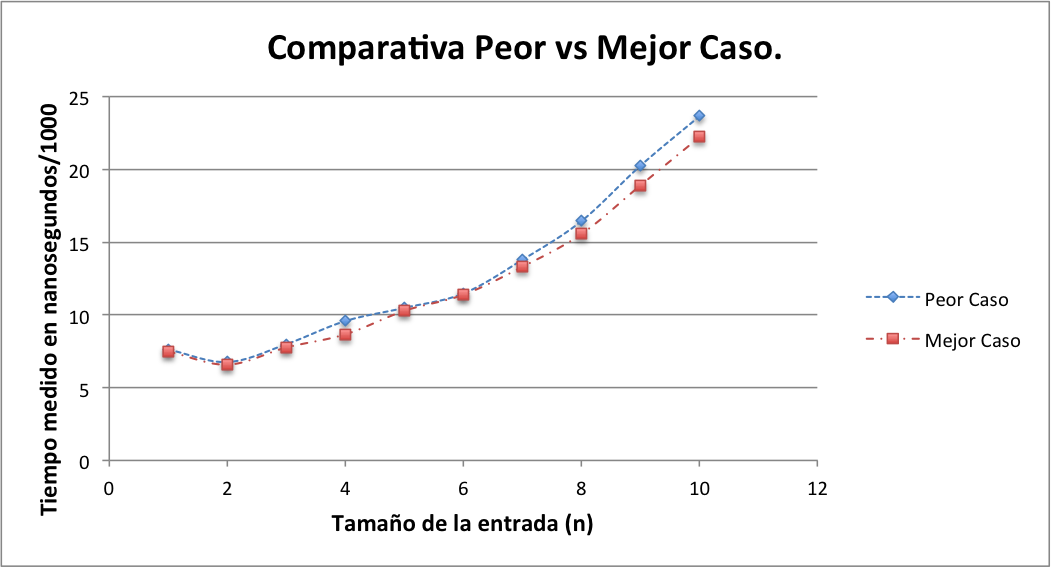
\includegraphics[width=140mm]{ejercicio3_mejorvspeor.png}
\centering
\caption{Comparativa Peor vs Mejor Caso}
\label{overflow3}
\end{figure}

\pagebreak

En el siguiente grafico pudimos realizar una acotacion de nuestro algoritmo. Por lo que pudimos acotarla por  $\bigO(e!)$ por debajo y
$\bigO(e!*(e^2))$ por arriba.

\begin{figure}[h!]
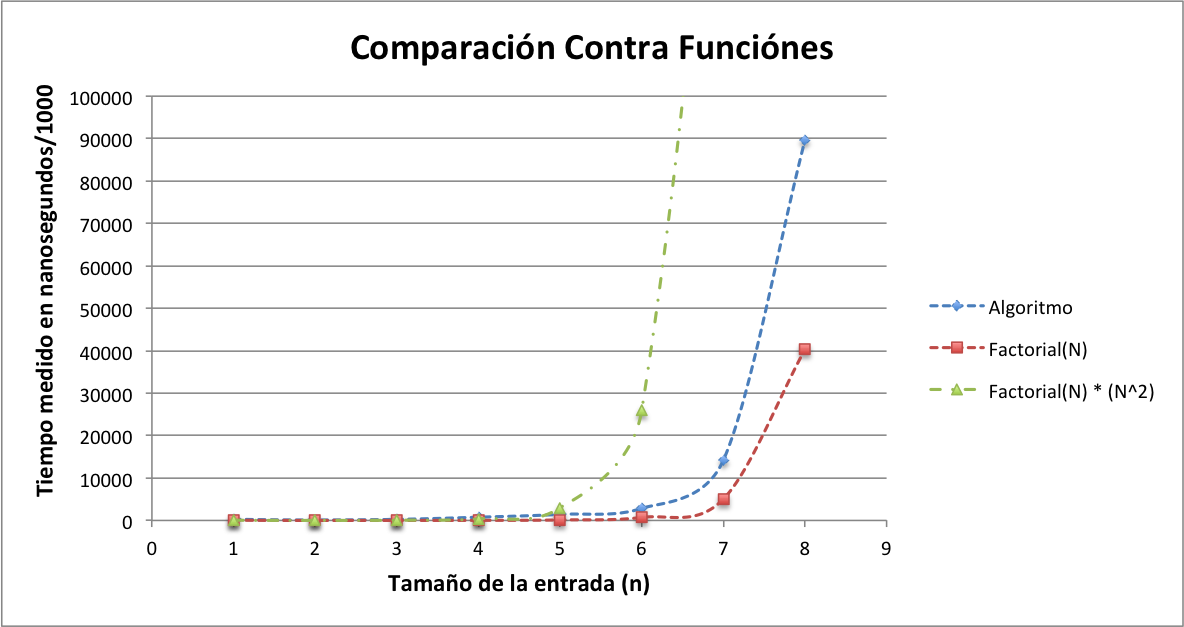
\includegraphics[width=140mm]{ejercicio3_comparacion_funciones.png}
\centering
\caption{Comparativa Contra Funcion Lineal y Cuadratica}
\label{overflow3}
\end{figure}

